%!TEX root = ../Bachelorseminar-RoboticSwarms.tex
	\begin{figure}[!ht]
		\caption{Venn Diagram; overview of algorithms}
		\label{venn_diagram}

		\centering

		\def\loclb{(180:2.0cm) circle (2.0cm)}
	  	\def\loclf{(0:2.0cm) circle (2.0cm)}
	  	\def\locrb{(90:2.0cm) circle (2.0cm)}
	  	\def\locrf{(270:2.0cm) circle (2.0cm)}

	    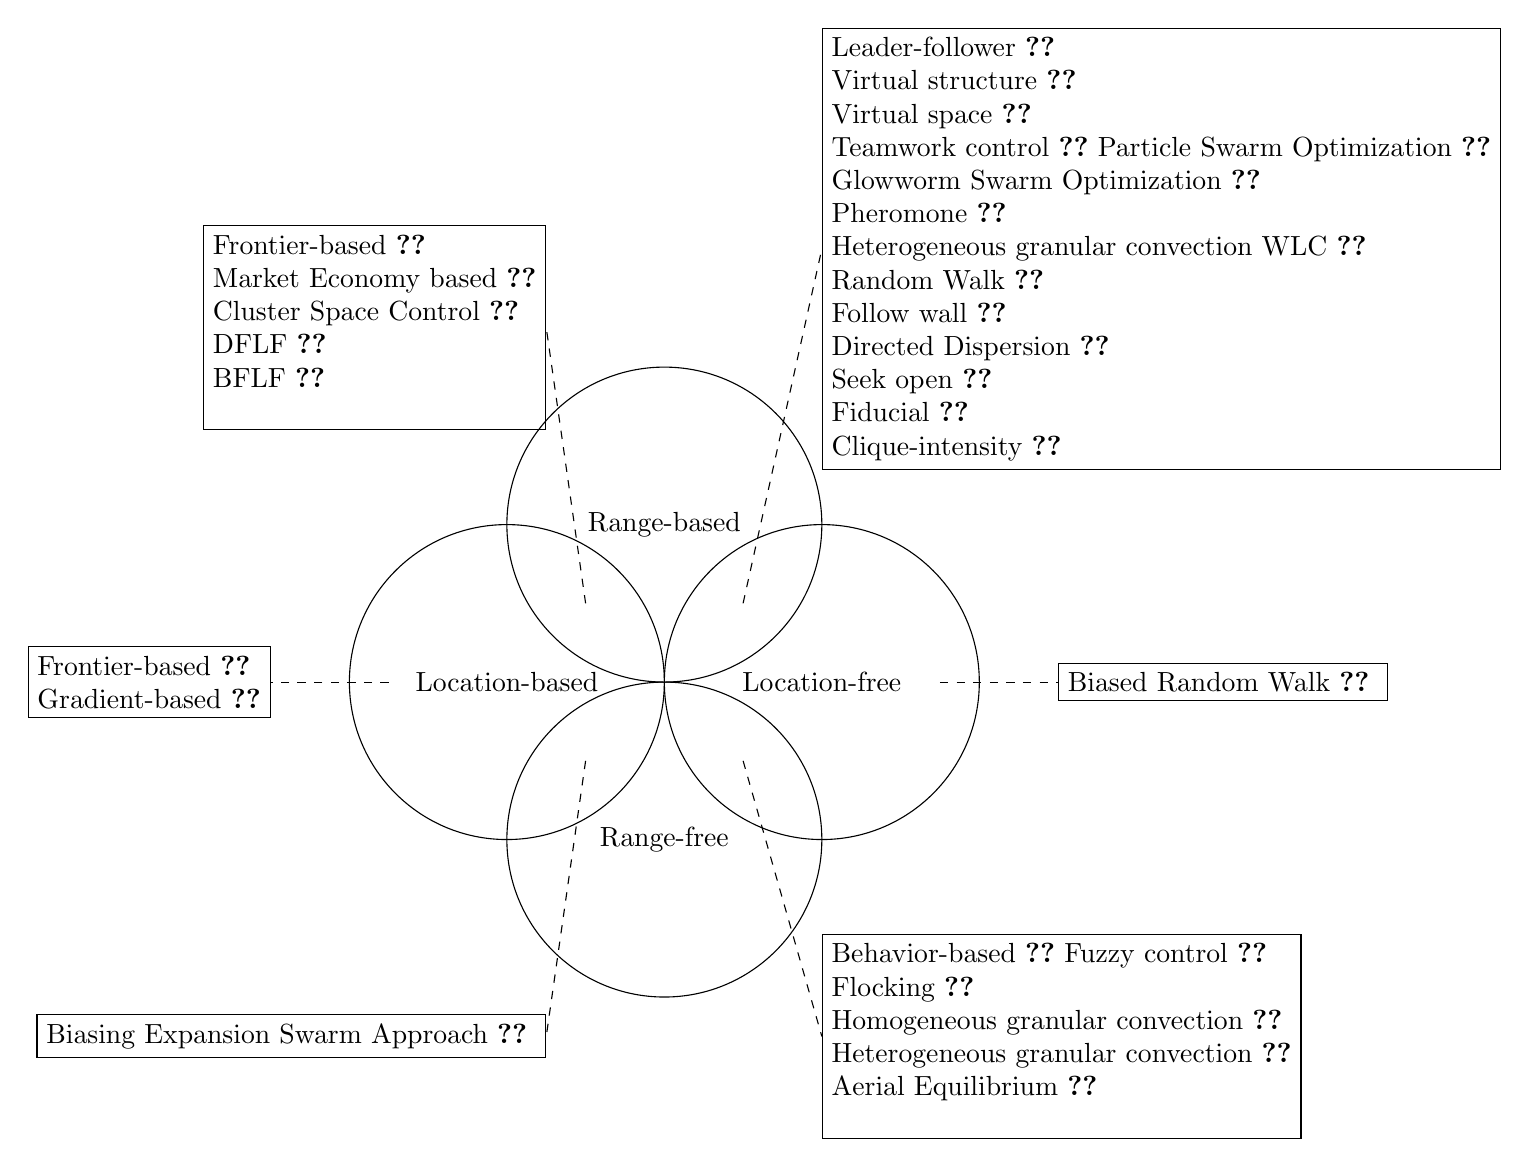
\begin{tikzpicture}
			% standard figures
			\draw \loclb node [text=black] {Location-based};
			\draw \loclf node [text=black] {Location-free};
			\draw \locrb node [text=black] {Range-based};
			\draw \locrf node [text=black] {Range-free};

			% Range-based location-free
			\draw[dashed,-] (1,1) -- (2,5.5) node[anchor=north west] {};
			\node[draw,align=left,anchor=west] at (2,5.5) {
				Leader-follower \ref{sec:Formation}\\
				Virtual structure \ref{sec:Formation}\\
				Virtual space \ref{sec:Formation}\\
				Teamwork control \ref{sec:Formation}
				Particle Swarm Optimization \ref{sec:Localization}\\
				Glowworm Swarm Optimization \ref{sec:Localization}\\
				Pheromone \ref{sec:CollectiveTransport}\\
				Heterogeneous granular convection WLC \ref{sec:CollectiveTransport}\\
				Random Walk \ref{sec:Dispersion}\\
				Follow wall \ref{sec:Dispersion}\\
				Directed Dispersion \ref{sec:Dispersion}\\
				Seek open \ref{sec:Dispersion}\\
				Fiducial \ref{sec:Dispersion}\\
				Clique-intensity \ref{sec:Dispersion}
			};

			% Range-free, location-free
			\draw[dashed,-] (1,-1) -- (2,-4.5) node[anchor=north west] {};
			\node[draw,align=left,anchor=west] at (2,-4.5) {
				Behavior-based \ref{sec:Formation}
				Fuzzy control \ref{sec:Formation}\\
				Flocking \ref{sec:CollectiveTransport}\\
				Homogeneous granular convection \ref{sec:CollectiveTransport}\\
				Heterogeneous granular convection \ref{sec:CollectiveTransport}\\
				Aerial Equilibrium \ref{sec:CollectiveTransport}\\
				%Virtual Pheromone \ref{sec:Path-planning}\\
				%Cardinality \ref{sec:Path-planning}
			};

			% location-free
			\draw[dashed,-] (3.5,0) -- (5,0) node[anchor=north west] {};
			\node[draw,align=left,anchor=west] at (5,0) {
				Biased Random Walk \ref{sec:Localization}
			};

			% location-based
			\draw[dashed,-] (-3.5,0) -- (-5,0) node[anchor=north west] {};
			\node[draw,align=left,anchor=east] at (-5,0) {
				Frontier-based \ref{sec:Exploration}\\
				Gradient-based \ref{sec:Localization}
			};

			% Range-free, location-based
			\draw[dashed,-] (-1,-1) -- (-1.5,-4.5) node[anchor=north west] {};
			\node[draw,align=left,anchor=east] at (-1.5,-4.5) {
				Biasing Expansion Swarm Approach \ref{sec:Localization}
			};

			% Range-based, location-based
			\draw[dashed,-] (-1,1) -- (-1.5,4.5) node[anchor=north west] {};
			\node[draw,align=left,anchor=east] at (-1.5,4.5) {
				Frontier-based \ref{sec:Exploration}\\
				Market Economy based \ref{sec:Exploration}\\
				Cluster Space Control \ref{sec:CollectiveTransport}\\
				DFLF \ref{sec:Dispersion}\\
				BFLF \ref{sec:Dispersion}\\
				%Artificial Bee Colony \ref{sec:Path-planning}\\
				%Multihop Communication \ref{sec:Path-planning}\\
				%Genetic Programming \ref{sec:Path-planning}
			};

			% Range-based
			%\draw[dashed,-] (0,3) -- (0,4.5) node[anchor=north west] {};
			%\node[draw,align=left,anchor=south] at (0,4.5) {

			%};

			% Range-free
			%\draw[dashed,-] (0,-3) -- (0,-4.5) node[anchor=north west] {};
			%\node[draw,align=left,anchor=north] at (0,-4.5) {
			
			%};
		\end{tikzpicture}
    \end{figure}

In the previous sections, we reviewed the main problems found in the field of robotic swarms. 
However, these problems often overlap.
This is because most of the problems found in robotic swarms often consist of multiple different problems. 
We focused on each main problem, highlighting the communication methods of every solution and properties of these communication methods. 
We summarize these properties in a Venn-diagram in figure~\ref{fig:AlgorithmsOverview}, allowing for a compact overview of these solutions.
The algorithms we discussed in previous sections provide useful insight, from which we can derive several conclusions.
Together with the Venn-diagram, we explain how we came to these conclusions. \\

\textbf{Location-based conclusions} 

\emph{Location-based} approaches keep track of some kind of map in such a way that the exact location of each swarm robot is accurately known.
Because of this, location-based approaches are often able to act efficiently and remove redundancy.
However, a couple of drawbacks can be defined.\\
\\
If an algorithm is \emph{location-based} and \emph{range-based}, the robots can create some kind of ad-hoc network to have global communication possibilities.
This global communication is very useful for exact orders and robot movement. 
But, such an ad-hoc network has a limited range. 
So, robots in the swarm can not split up from the rest of the groups to work outside this range. 
This takes away one of the great possibilities of robotic swarms decrease performance. \\
A robotic swarm can also accept that they do not have global communication.
Then, they can only share their map knowledge or location history with their neighbors, which will decrease performance.  \\
\\
In \emph{location-based} and \emph{range-free} algorithms, the robots can communicate via some central base, but not locally. 
This can increase performance dramatically, because redundancy in communication can be removed completely.
This is caused by the fact that every robot has access to all location information of all robots.
However, this will result in very low scalability, since the reliability of the central communication is entirely dependent on the capacity of the central base.

\textbf{Location-free conclusions} 

\emph{Location-free} approaches do not keep track of a map and are only able to determine some kind of relative position to each.
Alternatively they do not keep track of locations at all. 
This means they are able to optimally adapt to dynamic environments and can be implemented in low-level robots with cheap sensors. \\
\\
When an algorithm is both \emph{location-free} and \emph{range-free}, there generally exists no form of coordination. 
These algorithms are called collective algorithms and are often based on stochastic parameters. 
These robots all have distributed algorithms, but are often heterogeneous to carry out different tasks.
These algorithms are often highly scalable, because of the low communication overhead and cheap robots. 
Because they are highly scalable, many robots can exist in a swarm, and will eventually execute a task faster than a single robot.\\
\\
The majority of the algorithms that we discuss are \emph{location-free} and \emph{range-based}.
The main reason for this is that the algorithms mentioned in this category are very often highly scalable, have great performance and can be implemented with very simple robots. 
The difference with \emph{range-free} algorithms however is that in \emph{range-based} algorithms there exists some form of local communication.
This can increase the efficiency of such an algorithm dramatically, because the versatility of the swarm increases.
The robots can for example choose tostay together and share the information they get from their sensors, but can also choose to spread out in different groups to divide tasks depending on sensoral input. 
Because these algorithms are so versatile, they are well-suited for many different real-life applications.\\
\\
Finally, we acknowledge that we do not discuss many other problems found in robotic swarms. 
Examples include problems like the surveillance problem, as in how can a defined area effectively patrolled. 
Or the mapping problem, as in how a map of an area can be made efficiently. 
The reason we did not include these problems is because these are mostly all composite problems, of which we already have described their subproblems.
So, these sections would be redundant and would contribute little. \\
These omposite problems are closer to the application field of robotic swarms.
For future research, these composite problems could be expanded upon, focusing more on the application aspect. 

% As can be concluded from the diagram, most algorithms are location-free.
% This makes sense, as location-based are not the most desirable, although they do provide high performance.
% This is mainly because of three reasons. 
% The first reason is cost. 
% When an algorithm is location-based and range-based, the robots used in the swarm generally have to be equipped with advanced sensors. 
% The robots are then more costly in terms of energy consumption and device price, which is not desirable.
% The second reason is scalability. 
% When an algorithm is location-based, in most cases centralized communication is needed. 
% This introduces a lot of overhead, decreasing communication speed when robotic swarms increase in size. 
% The third reason is that algorithms that are location-based can often not be used in dynamic locations, like underwater, space and underground environment.
% This is especially true for algorithms where the operating environment has to be defined beforehand.\\
% \\
% Furthermore we have made the following observation about range usage and location usage. 
% When using a location-free approach, the algorithm easily adapts to dynamic environments.
% A downside to this approach is that the robots in this swarm can not know exactly what absolute location they have.
% This is why some algorithms chooose for a location-based approach. \\
% Some downside is that this approach can require central communication, which makes the scalability relatively low.
% In contrast when using a location-based approach, the robots can very accurately construct solutions out of their absolute location. 
% But, this can often not be implemented in a dynamic environment. 
% When using a location-based approach, we observe very optimal solutions, however these solution only remain to be optimal if the algorithm is used in a static environment. 
% Otherwise some basic algorithms such as collision-detection algorithms have to kick in, which can increase the overall runtime of the algorithm. Range-based algorithms allow for very dynamic environments and is one of the most important approaches due to its extreme usage of distributed intelligence. 

% Range-free algorithms on the other side are not very scalable and do not make use of efficient cooperation.

% This survey only highlighted a few problems that the robotic swarms technology has faced. 

% Thus, more research on this topic needs to be undertaken on additional problems, such as mapping, foraging, target localization and robot localization, in order to create a fully comprehensive overview.

% - voornamelijk location-free
%     - want maps moeten gemerged, bijgehouden worden gedeeld...

% - location-based voornamelijk exploration algoritmes
%     range-free location-free -> goed omdat gebruik bijv van wireless intensity signals erg onnauwkeurig is, non-optimal use of full robotic swarm
%     range-based location-free -> want maps moeten gemerged, bijgehouden worden gedeeld... en dynamische omgeving kan in de gaten gehouden worden
%     range-based -> belangrijkste gedeelte van een swarm, omdat daar de distributed intelligence ligt en dat daar het meeste onderzoek naar gedaan moet worden
%     location-based -> kan ook handig zijn in statische locaties, als er rekening gehouden wordt met de scalability van de swarm  
%     range-free -> matig scalable, maakt niet gebruik van efficiente samenwerking
% - range-based n range-free
